%%%%%%%%%%%%%%%%%%%%%%%%%%%%%%%%%%%%%%%%%%%%%%%%%%%%%%%%%%%%%%%%%%%%%%
% Overleaf (WriteLaTeX) Example: Molecular Chemistry Presentation
%
% Source: http://www.overleaf.com
%
% In these slides we show how Overleaf can be used with standard 
% chemistry packages to easily create professional presentations.
% 
% Feel free to distribute this example, but please keep the referral
% to overleaf.com
% 
%%%%%%%%%%%%%%%%%%%%%%%%%%%%%%%%%%%%%%%%%%%%%%%%%%%%%%%%%%%%%%%%%%%%%%

\documentclass{beamer}

\mode<presentation>
{
  \usetheme{Madrid}       % or try default, Darmstadt, Warsaw, ...
  \usecolortheme{default} % or try albatross, beaver, crane, ...
  \usefonttheme{default}    % or try default, structurebold, ...
  \setbeamertemplate{navigation symbols}{}
  \setbeamertemplate{caption}[numbered]
} 

\usepackage[english]{babel}
\usepackage[utf8x]{inputenc}
\usepackage{chemfig}
\usepackage[version=3]{mhchem}

\usepackage{hyperref}
  \hypersetup{colorlinks=true}
  \hypersetup{urlcolor=blue}
  \hypersetup{linkcolor = .}
\usepackage{xcolor}
\usepackage{siunitx}
  \sisetup{separate-uncertainty = true}
\usepackage{physics}
\usepackage[font=small,labelfont=bf]{caption}
\usepackage{subcaption}
\usepackage[en-GB]{datetime2}
\usepackage{feynmp}
\DeclareGraphicsRule{*}{mps}{*}{}

\usepackage{scalerel}
\newcommand{\mylbrace}[2]{\vspace{#2pt}\hspace{6pt}\scaleleftright[\dimexpr5pt+#1\dimexpr0.06pt]{\lbrace}{\rule[\dimexpr2pt-#1\dimexpr0.5pt]{-4pt}{#1pt}}{.}}
\newcommand{\myrbrace}[2]{\vspace{#2pt}\scaleleftright[\dimexpr5pt+#1\dimexpr0.06pt]{.}{\rule[\dimexpr2pt-#1\dimexpr0.5pt]{-4pt}{#1pt}}{\rbrace}\hspace{6pt}}

% Here's where the presentation starts, with the info for the title slide
\title[BESIII Oxford]{BESIII Oxford Group Meeting}
\author{Martin Tat}
\institute{Oxford LHCb}
\date{\today}

\titlegraphic{
\includegraphics[width = 5cm, height = 3.8cm]{lhcb.jpg}\hspace{1cm}~%
              
\includegraphics[width = 5cm, height = 3.8cm]{bes3.png}}

\begin{document}

\begin{frame}
  \titlepage
\end{frame}

% These three lines create an automatically generated table of contents.
%\begin{frame}{Outline}
%  \tableofcontents
%\end{frame}

\section{Introduction}
\begin{frame}{Introduction}
  \begin{itemize}
    \item{Aim: Measure $c_i$ and $s_i$ in the decay $D\to K^+K^-\pi^+\pi^-$, $D = D^0, \bar{D^0}$}
    \item{End goal: Model independent binned analysis to measure $\gamma$ at LHCb}
    \item{So far:}
    \begin{itemize}
      \item{Familiarized myself with BOSS and BESIII analysis}
      \item{Ran a single tagging on $~2\%$ of the $2010$ MC inclusive sample ($20x$ luminosity)}
      \item{Sorted events into signal and background categories}
    \end{itemize}
  \end{itemize}
\end{frame}

\section{Initial single tagging}
\begin{frame}{Initial single tagging}
  \begin{figure}
    \centering
    \begin{subfigure}{0.5\textwidth}
      \centering
      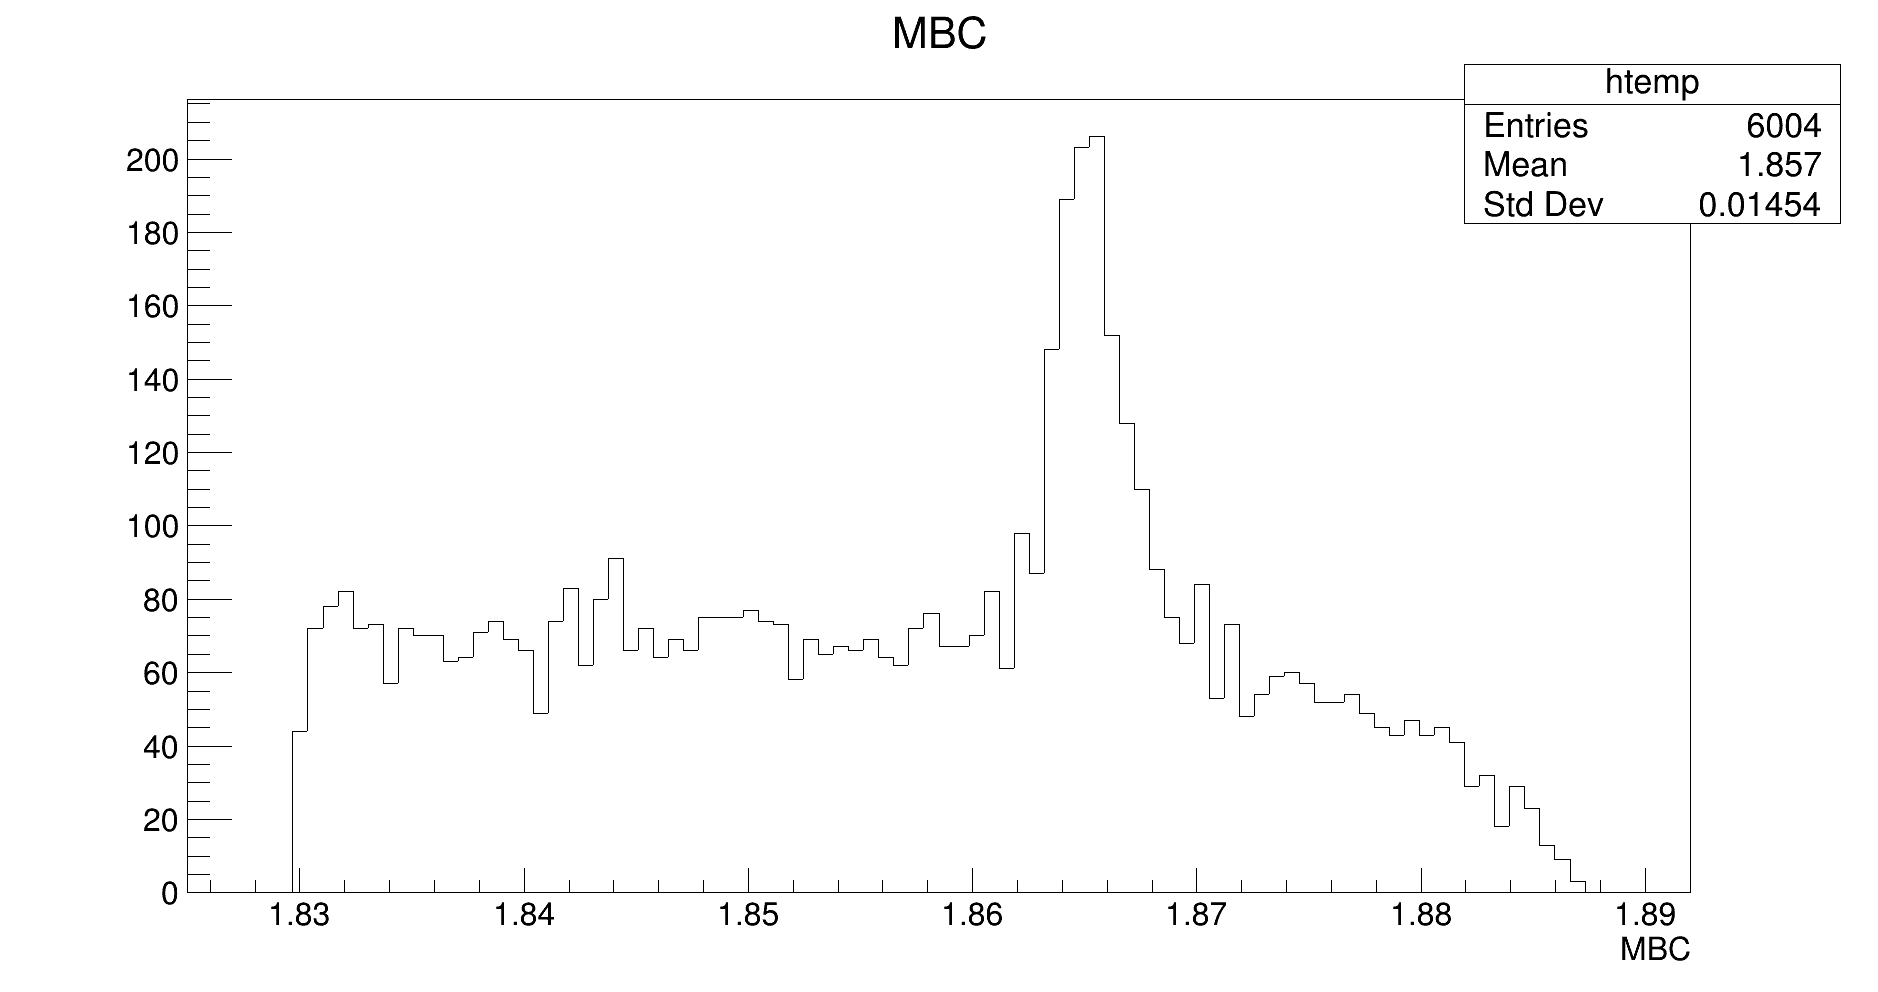
\includegraphics[width=\textwidth]{MBC.png}
      \caption{$m_{BC}$, beam constrained mass}
    \end{subfigure}%
    \begin{subfigure}{0.5\textwidth}
      \centering
      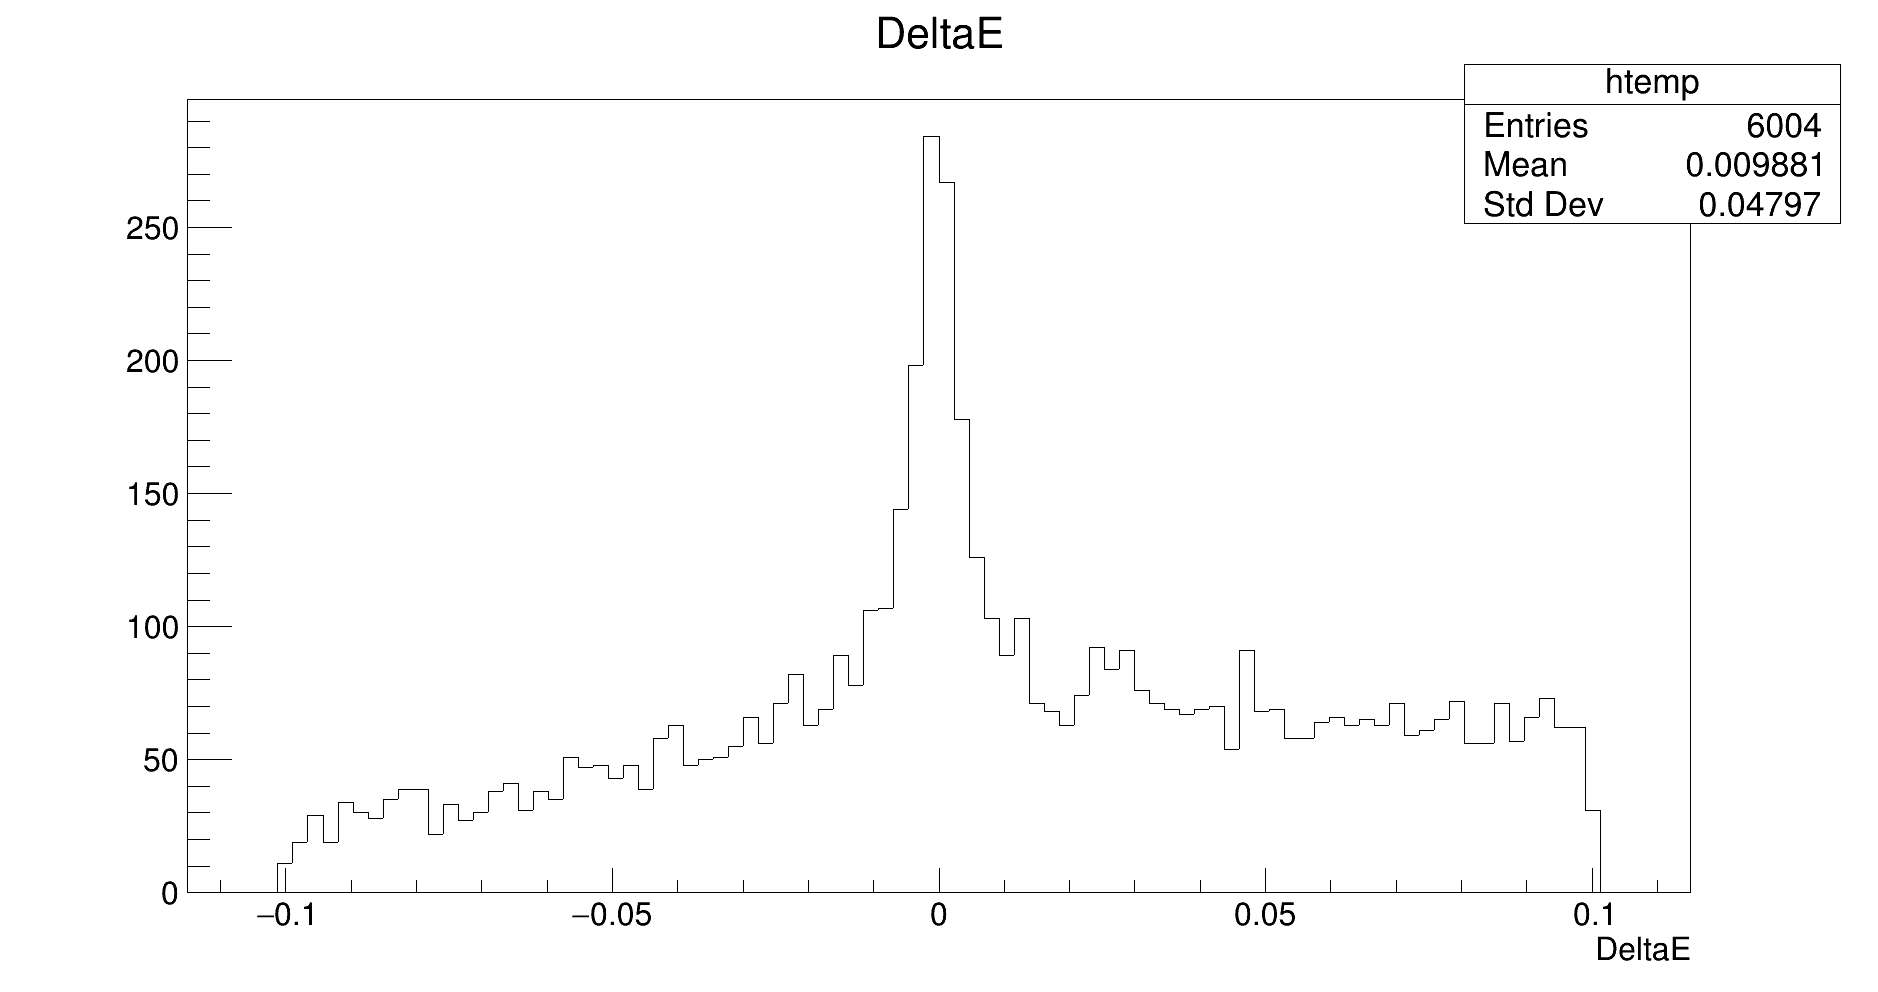
\includegraphics[width=\textwidth]{DeltaE.png}
      \caption{$\Delta E$, missing energy}
    \end{subfigure}
    \caption{Initial single tagging}
  \end{figure}
\end{frame}

\begin{frame}{Next steps}
  \begin{itemize}
    \item{Double tags (which tag modes should I use?)}
    \item{$K_S^0$ reconstruction?}
    \item{Detailed study of background}
  \end{itemize}
\end{frame}

\end{document}
